\section{Evaluation}
\softner{} solves the problem of entity recognition and extraction from unstructured text descriptions of incidents. But to evaluate the \softner{} framework in its entirety, we propose a 3 phase evaluation, to assess \softner{}'s applicability to incident management. We thus, answer the following questions using the evaluation:
\begin{itemize}
    \item \textbf{Entity Types}: How does \softner{}'s unsupervised approach perform in recognizing distinct entity types?
    \item \textbf{SoftNER Model}: How does the \softner{}'s Multi-Task model compare to state-of-the-art deep learning approaches for the NER task?
    \item \textbf{Auto-Triage}: Does \softner{} help improve the downstream task of automated incident triaging?
\end{itemize}

\subsection{Study Data}
\label{sec:study_data}
In the following evaluation experiments, we apply \softner{} to service incidents of \CompanyX{}, a major cloud service provider. These are incidents retrieved from large scale online service systems, which have been used by a wide distribution of users. In particular, we collected 41,000 incidents spanning over a time period of 2 months. Each incident is described by its unique Id, title, description, last-modified date, owning team name and, also, whether the incident was resolved or not. Incident description is the unstructured text with an average of 472 words, showing us how verbose the incident descriptions are. Owning Team Name here, refers to the team to which the incident has been assigned.

\subsection{Entity Type Evaluation} 

Here, we evaluate the effectiveness of \softner{}'s unsupervised approach for named-entity extraction. Specifically, we evaluate the correctness of the entity types extracted by \softner{} on the entire study data of 41,000 incidents. As the component performs \textbf{unsupervised} information extraction, we manually evaluate the precision of extraction. The component, first, extracts 100 distinct entities  sorted by the frequency of occurrence. We then, manually validate each potential entity and perform analysis on precision. Precision, here, is the fraction of extracted entities that are actually software entities.

Since the precision of \softner{}'s entity type extraction depends on the frequency of occurrence of entities, we further plot precision against a cut off rank $n$. Figure \ref{pattern-extraction} summarizes the precision of \softner{}'s entity type extraction against the top $n$ entities extracted, where $n \in [1,100]$. From this analysis, we see that \softner{} is able to extract 77 valid entities per 100 entities. We also see an expected decrease in precision, as $n$ increases, due to noisy tokens (false positives) like \textit{"to troubleshoot issue"}, \textit{"for cleanup delay"} and \textit{"for application gateway"}.

As explained above, in performing this experiment, n corresponds to the rank of the entity extracted. That is, a higher $n$ refers to an entity with low frequency of occurrence, which in turn can be extrapolated as an entity that is less important. \softner{}'s unsupervised entity type extraction has a minimal precision variation, also known as fall out rate, of 0.23 for an $n$ value as high as 100. This strengthens the hypothesis that \softner{}'s pattern extractors can pick up entities from unstructured text effectively, in a completely unsupervised manner.  

\begin{figure}%[H]
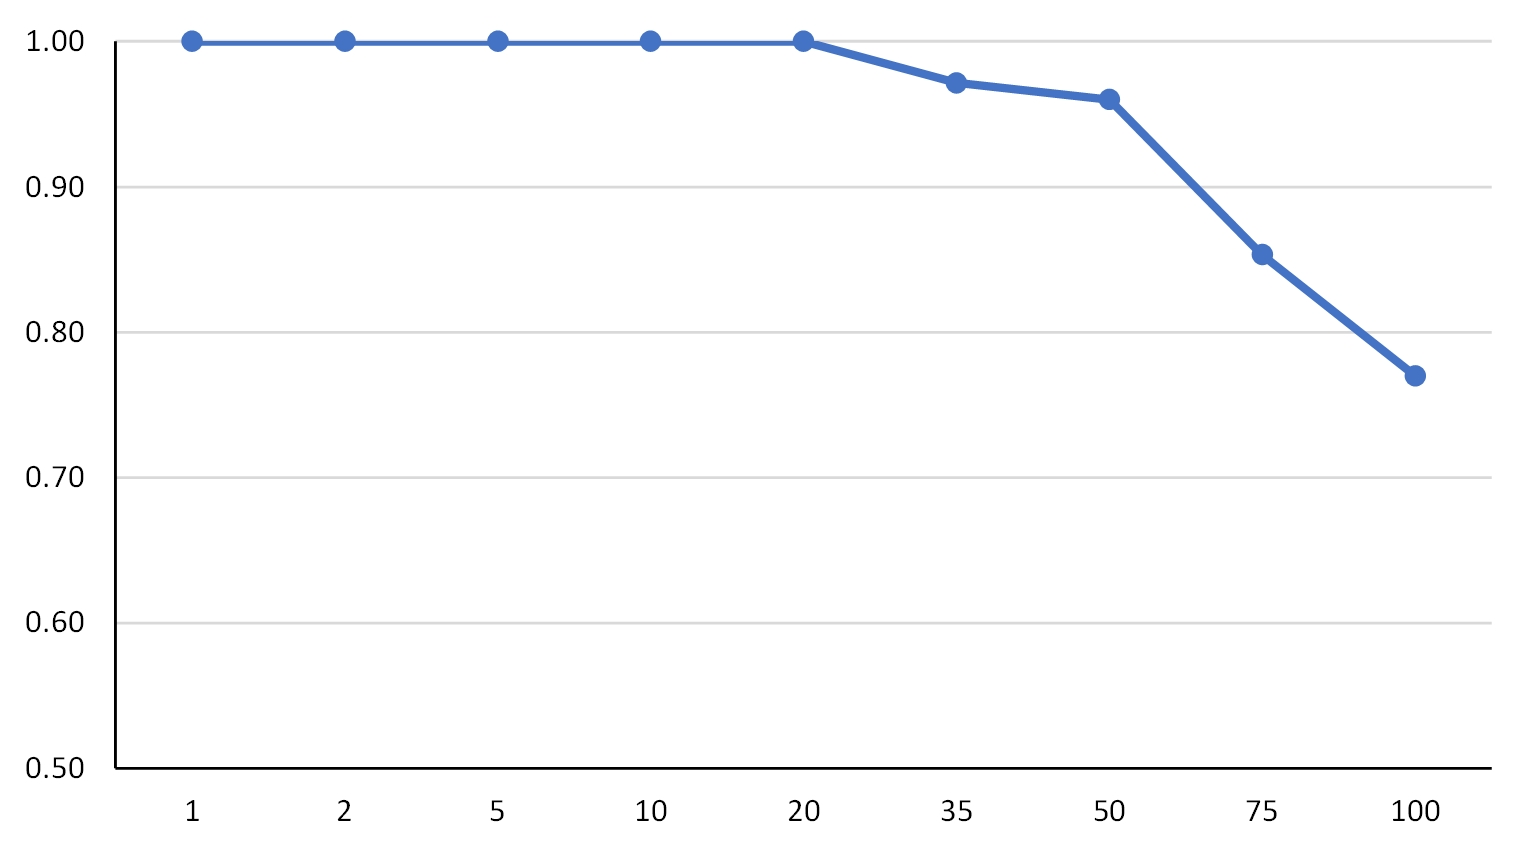
\includegraphics[width=\linewidth]{Figures/pattern_extraction_eval.jpg}
\caption{Precision vs Rank curve for the entity types}
\label{pattern-extraction}
%\vspace{-6pt}
\end{figure}

\subsection{\softner{} Model Evaluation}
Here, we evaluate the SoftNER deep learning model on the Named-Entity Recognition Task. We compare the multi task model, described in section \ref{sec:multi-task-model} and Figure \ref{model-arch}, against two baseline models, BiLSTM-CRF and BiLSTM-CRF with attention mechanism. These baseline models are state-of-the-art for NER \cite{huang2015bidirectional,lample2016neural, chiu2016named} and other NLP tasks as well. The models are compared on a fixed test set with 8300 incidents, that accounts for $20\%$ of the data-set. We use average precision, recall and F1 metrics to evaluate and compare the models on the NER task. The metrics are averaged over around 70 distinct type of entities tagged by the model. We also use a version of the F1 score, weighted based on the support for individual entities.

As shown in Table \ref{model-evaluation}, we observe that the baseline BiLSTM-CRF, with and without attention mechanism, achieves an average F1 score of around 0.88. Whereas, \softner{}'s Multi Task Model, as described in Section \ref{sec:multi-task-model}, achieves a higher average F1 score of around 0.96, i.e., a $\Delta F1\%$ of 8.7\%. \softner{} deployed as a solution in the incident management environment, is required to extract as much information from incident descriptions as possible. This is because, more information directly correlates with the ease of understanding the problem and identifying resources affected by the incident. We evaluate this ability using recall metrics and observe a high average recall of 0.95, as shown in Table \ref{model-evaluation}.

We further analyze the generalization of the model by analyzing test examples that were either false positive or false negative. Table \ref{false-examples} shows a few examples of sentences and the entities extracted from them. Note that we refer to false positives as FP, and, false negatives as FN in the table. We observe that some of the FPs are actually correct and were mislabelled in the test set because of the limitations of the pattern extractors. Let's take Example 1 from Table \ref{false-examples} for instance. Here, the unsupervised labelling component was only able to label \textbf{\textit{"2aa3abc0-7986-1abc-a98b-443fd7245e6"}} as \textbf{Subscription Id}, but not \textbf{\textit{"vaopn-uk-vnet-sc"}} as \textbf{Vnet Name} in the test sentence, due to restrictions with pattern extractors and label propagation. But the \softner{} model was able to extract both the entities from the sentence, proving it's ability to generalize beyond obvious structural pattern rules visible in the training data. In another example, row 2 in Table \ref{false-examples}, \textbf{403} was tagged \textbf{Error Returned} and \textbf{200} as \textbf{Status Code}, even though no structural elements (like ":") were present in the description. Row 3 shows a similar false positive example with the extraction of \textbf{\textit{192.168.0.5}} as \textbf{IP Address}. We also show a few contrasting false negatives, in rows 4 and 5, where the model was unable to extract entities \textbf{Ask} and \textbf{Ip Address} respectively.

\begin{table}
\small
\caption{Model evaluation}\vspace{-6pt}
\label{model-evaluation}
 \begin{tabular}[t]{lccc} 
\toprule
 \textbf{Metric} & \textbf{BiLSTM-CRF} & \textbf{BiLSTM-CRF} & \textbf{SoftNER} \\
  &  & \textbf{ Attention} & \textbf{Model} \\
 \midrule
 Avg F1 & 0.8803 & 0.8822 & \textbf{0.9572} \\
 Weighted Avg F1 &  0.9401 & 0.9440 & \textbf{0.9682} \\
 Avg Precision & 0.9160 & 0.9088 & \textbf{0.9693} \\
 Avg Recall &  0.8669 & 0.8764 & \textbf{0.9525} \\
 \bottomrule
\end{tabular}
\end{table}

\begin{table}
\small
\caption{FP and FN examples}\vspace{-6pt}
\label{false-examples}
\begin{tabular}[t]{ p{4cm} c p{2cm}} 
\toprule
\textbf{Sentence} & \textbf{Evaluation} & \textbf{Entities Tagged}\\
 & \textbf{Result} & \\
\midrule
\textit{SubscriptionId : 2aa3abc0-7986-1abc-a98b-443fd7245e6 unable to delete vnet name vaopn-uk-vnet-sc} & FP & {2aa3abc0-7986-1abc-a98b-443fd7245e6, vaopn-uk-vnet-sc }\\

\textit{Customer is reporting that their alerts for div-da are firing as 403 errors when the service is fully up and running with 200 codes} & FP & {403, 200} \\

\textit{Device Name : njb02-23gmk-isc, pa: 192.168.0.5 could not be configured! Error!} & FP & {njb02-23gmk-isc, 192.168.0.5} \\

\textit{The customer's  main ask: Need help to access cloud storage from cloud hosted service}  & FN & - \\

\textit{The loopback (ipv4) address (primary) is 192.131.75.235} & FN & {ipv4} \\
\bottomrule
\end{tabular}
\end{table}

\subsection{Auto-Triaging of incidents}
Incident triaging refers to the process of assigning a new incident to the responsible team. This is currently manually performed by the on-call engineers and it is not uncommon for the incident to be reassigned to a different team at a later point thereby reducing the accuracy and efficiency of incident management. These incidents often lead to huge economic losses and dissatisfaction amongst customers. Based on an empirical study, Chen et al. \cite{EmpiricalIcMICSE2019} showed that the reassignment rate for incidents can be as high as 91.58\% for online services at Microsoft. This shows the importance of incidents being assigned to the correct team at creation time. Several efforts \cite{EmpiricalIcMICSE2019, ContinuousTriageASE2019} have been made to automate the triaging process by leveraging the title, description and other meta-data of the incidents. Here, we evaluate the effectiveness of the knowledge extracted by \softner{} for the downstream task of automated triaging of incidents. Incident triaging is essentially a multi-class classification problem since the incident could be assigned to one of many teams. 

We sample $8000$ resolved incidents for the $10$ most common teams from the initial $41,000$ incident set (refer Section \ref{sec:study_data}) and run the \softner{} model on the description to extract the entities. The \softner{} entities can be broadly classified as either categorical or descriptive. While the descriptive entities are transformed to word embeddings using the same process described in Section \ref{sec:glove-word-emb}, the categorical entities are encoded into one-hot vectors. We then look at different combinations of features and compare the 5 fold cross-validation accuracy on various classification models. It is evident from Table \ref{tab:auto-triaging-models} that the models using the \softner{} entities, either on their own or along with the title, outperform the baseline models that use only the title and description information. We observe significant margins, with up to $7$\% - $27$\% increase in the 5 fold cross validation accuracy scores. These results reinforce that the entities extracted by \softner{} are indeed useful and can significantly help in downstream tasks. Using the entities extracted by \softner{} also reduces the input feature space since we no longer have to use the whole incident description. We also achieve high performance models using simple machine learning models thereby eliminating the need for complex deep learning models which have proven to be superior in past studies \cite{EmpiricalIcMICSE2019}.

In addition to comparing the cross validation accuracy of different models, we analysed feature significance by using the feature\_importances\_ attribute of a random forest model trained on the various input features. We observed that the entities extracted by \softner{} were given far more importance compared to the `Title', with the top features being - `exception message',  `problem type', `ask' and `issue' (as shown in Table \ref{tab:feature_significance}). This re-emphasises that the entities extracted from \softner{} boost the performance of classification models for the downstream task of automatic triaging of incidents.


\begin{table}
\small
    \begin{center}
    \caption{Comparison of 5 fold cross validation accuracy for auto-triaging using different feature sets.}
    \label{tab:auto-triaging-models}
    \vspace{-6pt}
    \setlength\tabcolsep{2 pt}
    \begin{tabular}{@{}p{2.66cm}ccccc@{}}
        \toprule
        %\textbf{Feature Set}  & \textbf{Random Forest} & \textbf{Linear SVM} & \textbf{Gaussian SVM} &  \textbf{K-Nearest Neighbors} & \textbf{Naive Bayes} \\ 
         
        \textbf{Feature Set}  & \textbf{Random} & \textbf{Linear} & \textbf{Gaussian} &  \textbf{K-Nearest} & \textbf{Naive} \\[-2pt]
         & \textbf{Forest} & \textbf{SVM} & \textbf{SVM} & \textbf{Neighbors} & \textbf{Bayes}\\
        \midrule
        Title + Description & 74.64 & 85.93 & 87.06 & 81.32 & 69.69 \\
        \midrule
        \softner{} Entities & 93.38 & 93.34 & 93.39 & 92.40 & 87.67\\
        $\Delta$ \% & 22.31 & 8.26 & 7.02 & 12.76 & 22.85 \\
        \midrule
        \softner{} Entities + Title & \textbf{98.60} & \textbf{99.20} & \textbf{98.95} & \textbf{99.14} & \textbf{88.07} \\
        $\Delta$ \% & 27.66 & 14.34 & 12.78 & 19.75 & 23.30 \\
        % $\Delta$ (Title + Summary,\newline \softner{} Entities + Title) & +23.96 & +13.27 & +11.89 & +17.82 & +18.38 \\
        %\softner{} + Title + Summary & 98.74 & 99.40 & 99.24 & 98.64 & 89.86\\
        
        \bottomrule
    \end{tabular}
    \end{center}
\vspace{-6pt}
\end{table}



\begin{table}[H]
\vspace{-6pt}
\small\centering
%    \begin{center}
    \caption{Importance scores for top features}
    \label{tab:feature_significance}
    \vspace{-6pt}
    \setlength\tabcolsep{2 pt}
    \begin{tabular}{lccccc}
        \toprule
        \textbf{Feature}  & Exception & Problem & Ask &  Issue & Title \\[-3pt]
        & Message & Type & & \\
        \midrule
        \textbf{Importance} & 0.0133 & 0.0111 & 0.0097 & 0.0051 & 0.0009\\
        \bottomrule
    \end{tabular}
%    \end{center}
\vspace{-6pt}
\end{table}